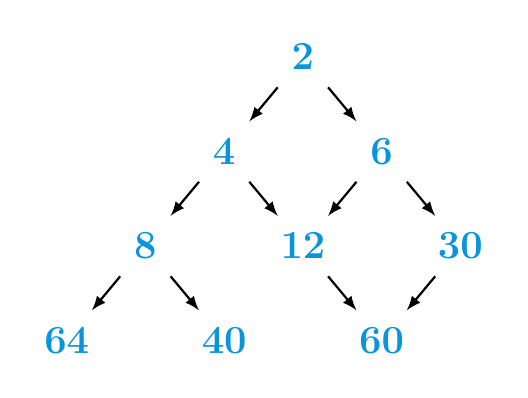
\begin{tikzpicture}[>=latex]

% --- Stijldefinities (gebaseerd op jouw aanpassingen) ---
\tikzset{
    getal/.style={
        text=cyan!80!blue, 
        font=\Large\bfseries, 
        inner sep=6pt
    },
    pijl/.style={
        ->,
        >=latex,
        thick,
        draw=black, 
        shorten >=0.1pt,      
        shorten <=0.1pt
    }
}

% --- Knooppunten (Nodes) ---

% Niveau 0 (Top)
\node[getal] (n2) at (0, 3.6) {2};

% Niveau 1
\node[getal] (n4) at (-1, 2.4) {4};
\node[getal] (n6) at (1, 2.4)  {6};

% Niveau 2
\node[getal] (n8)  at (-2, 1.2) {8};
\node[getal] (n12) at (0, 1.2)  {12};
\node[getal] (n30) at (2, 1.2)  {30};

% Niveau 3 (Bottom)
\node[getal] (n64) at (-3, 0) {64};
\node[getal] (n40) at (-1, 0) {40};
\node[getal] (n60) at (1, 0)  {60};


% --- Pijlen (van boven naar beneden) ---

% Verbindingen vanaf 2
\draw[pijl] (n2) -- (n4);
\draw[pijl] (n2) -- (n6);

% Verbindingen vanaf 4 en 6
\draw[pijl] (n4) -- (n8);
\draw[pijl] (n4) -- (n12);
\draw[pijl] (n6) -- (n12);
\draw[pijl] (n6) -- (n30);

% Verbindingen vanaf 8, 12 en 30
\draw[pijl] (n8) -- (n64);
\draw[pijl] (n8) -- (n40);
\draw[pijl] (n12) -- (n60);
\draw[pijl] (n30) -- (n60);

\end{tikzpicture}